\section{The R\lowercase{e}D Experiment}
\label{sec:Red}

The \ReD\ project aims to characterize the light and charge response of the \LArTPC\ to neutron-induced nuclear recoils, especially at low energy, and to explore for the possible directional dependence suggested by the \SCENE\  experiment~\cite{Alexander:2013ke,Cao:2015ks}. \ReD\ encompasses the irradiation of a miniaturized \LArTPC\ with a neutron beam at the INFN, Laboratori Nazionali del Sud (LNS), Catania. Neutrons are produced via the reaction p($^{7}$Li,$^7$Be) from a primary $^{7}$Li beam delivered by the TANDEM accelerator of LNS.  A $\Delta E/E$ telescope, made by two Si detectors, identifies the charged particles ($^{7}$Be) which accompany the neutrons emitted towards the \TPC. Neutrons scattered from the \TPC\ are detected by using an array of nine \RedLNSNeutronSpectrometerDetectorsPMTsDiameter\ liquid scintillator (LSci) detectors,  using \RedLNSNeutronSpectrometerDetectorsScintillatorType\ liquid scintillator coupled to \RedLNSNeutronSpectrometerDetectorsPMTsType\ \PMTs.  The \ce{Si} telescope and the \TPC\ are not at the same height: this is mandatory in order to tag neutron scatterings (n,n') from a non-horizontal interaction plane. All LSci are placed such to tag recoils having the same energy, i.e. the same scattering angle with respect to the incident neutron, but different angle with respect to the drift field of the \LArTPC, thus allowing to search for a possible directional response. Thanks to the support provided by INFN CSN2, the entire set-up has been procured, integrated, commissioned and deployed to the ``80 deg'' beamline of LNS. The first beam run test took place in June-July, 2018. 

The core detector of \ReD\ is a custom-made \TPC\ designed by UCLA, which is a miniaturized version of the \LArTPC\ for \DSks.  The \TPC\ is a cube with size of about \GAPTPCActiveDiameter.  An acrylic vessel defines the active volume, with the top and bottom acrylic windows \ITO\ coated to allow for the application of the electric field, and the side ESR-acrylic sandwich reflection panels to maximize the reflectivity of the chamber. All of the internal surfaces are coated with TPB to wavelength shift the argon scintillation light. The drift field is kept uniform along the drift coordinate by means of the field shaping rings, deposited by thin-coating the walls of the acrylic vessel with \ITO. The drift length, extraction length and electroluminescence length of the \ReD\ \TPC\ are 5~cm, 3~mm and 7~mm, respectively. The \ReD\ \TPC\ uses all the innovative features of the \DSks\ design, in particular the optoelectronic readout based on \SiPM\ developed by FBK and the cryogenic electronics. Two 5x5~cm$^2$ tiles are available from FBK, each made by 24 rectangular \SiPMs.  The tile on the top of the \LArTPC\ has a 24-channel readout, in order to improve the $(x,y)$ sensitivity, while the bottom tile has a standard 4-channel readout.  A dedicated 24-channel Front End Board (FEB) has been designed and produced by INFN-Na in collaboration with INFN-Bo and LNGS. 

The \LArTPC\ is contained in a new cryogenic system. The commissioning of the system was carried out in Naples. Starting from April 2018, the new \TPC\ and cryogenic system were operated and tested. Measurements were taken with lasers, low-energy $\gamma$ sources and neutrons from a DD generator. This allowed for the first characterization of the \LArTPC\ and for an integrated test of: operating procedures, photosensors, \DAQ, slow control, data handling and reconstruction algorithms. The system was successfully operated 
in single and double phase modes, with a light yield of about 10~phe/keV at null field. The new LabVIEW-based slow control developed by INFN-Genova was also integrated and commissioned. The set-up was irradiated in Naples with the DD neutron gun from the Temple University, such to assess the PSD performance of the \LArTPC. The run also included one LSci, allowing for the first test of the \DAQ\ for a system made by two different types of detectors. All nine LSci detectors had been previously tested and characterized at INFN-Roma1. 

The commissioning and the characterization of the system in Naples opened the way for the deployment of the system at the beamline of \LNS.  The entire set-up (\TPC\ with cryogenic system, liquid scintillators with their \PMTs\ and the mechanical support structure) was shipped and re-assembled in Catania in June 2018. Meanwhile, the beamline had been refurbished on the basis of the experimental design, optimized with dedicated Monte Carlo simulations, and the mechanical clearance requirements. The configuration was conceived to allow the tagging of nuclear recoils between 20 and 100~keV traveling in the parallel and orthogonal directions with respect to the \TPC\ drift field, by varying the primary beam energy only. Furthermore, having a dedicated liquid scintillator at small scattering angles opens the possibility to study the response of the \TPC\ to very low-energy nuclear recoils, O(1~keV).  A new scattering chamber was installed with a new beam pipe. The $\Delta E/E$ telescope was installed inside the vacuum scattering chamber, commissioned and consists of two Si detector (20 $\mu$m and 200 $\mu$m thickness, respectively) by ORTEC. 

Initially, the cryostat and the liquid scintillators had to be mechanically aligned with respect to the target with a precision of the order of a few mm. The alignment was performed by following a detailed procedure worked out in advance. The \ReD\ set up in Catania is displayed in Fig.~\ref{fig:BeamlinePhoto}. 

\begin{figure}[t!]
\centering
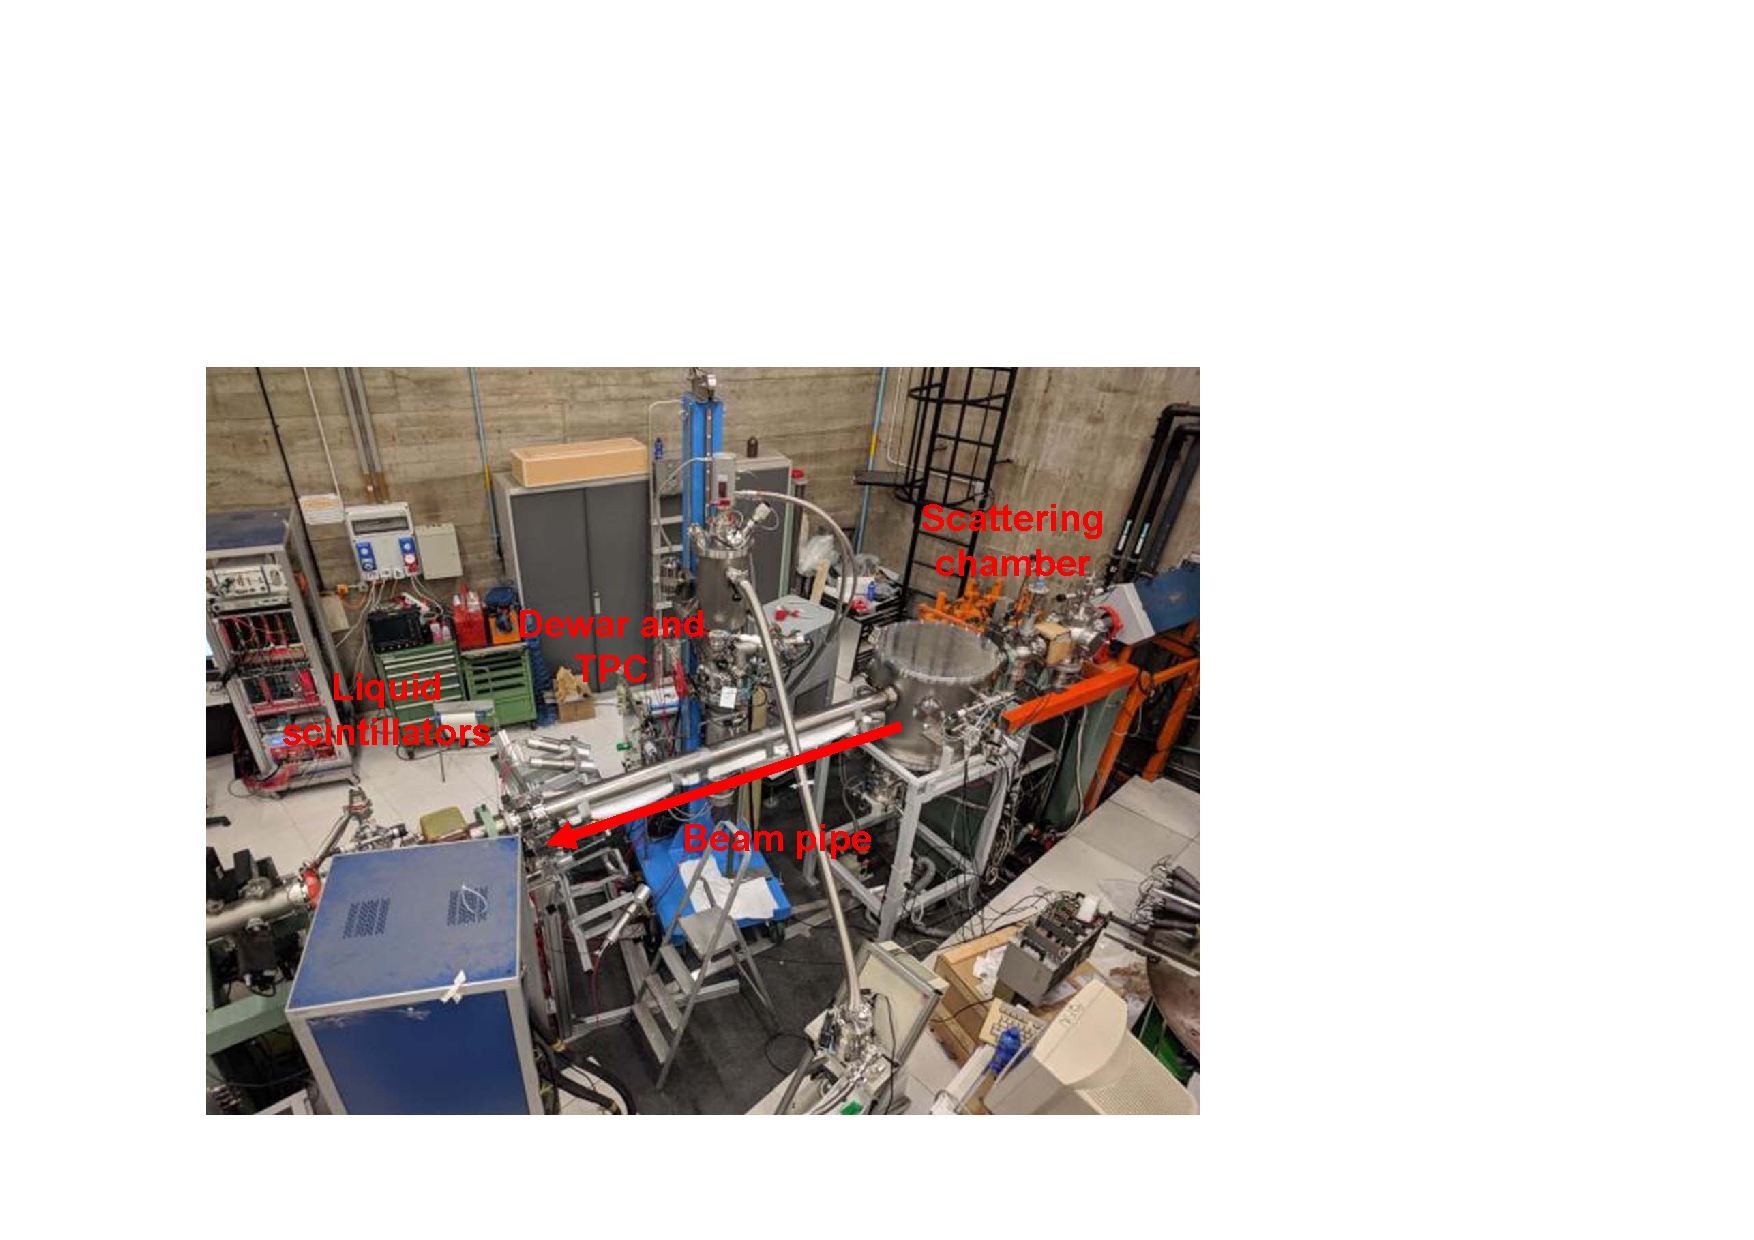
\includegraphics[width=\columnwidth]{./Figures/BeamLineDisplay.pdf}
\caption[Picture of the \LNS\ beamline in use for \ReD]{Photo of the ``80 deg'' beamline at \LNS, after the deployment and alignment of \ReD.  The targets and the Si telescope are hosted inside the vacuum scattering chamber.}
\label{fig:BeamlinePhoto}
\end{figure}

After the scientific approval of the project by the Scientific Committee (PAC) of \LNS, a test beam run was scheduled in June-July 2018, meant for technical tests and commissioning. The individual detectors were first commissioned and tested individually, by using the laser and radioactive sources. Light yield and timing were checked by using $^{241}$Am and $^{22}$Na, respectively.  A $^{252}$Cf fission neutron source was used to characterize the pulse shape discrimination performance of both the \LArTPC\ and the LSci detectors. The light yield of the \TPC\ was measured to be about 8.5~phe/keV, while the electron drift lifetime about 250~$\mu$s, i.e. much longer than the total drift time (about 40~$\mu$s at the operational field of 0.2~V/cm), with no hints of degradation in time. The calibration of the LSci detectors indicated a \SI{50}{\percent} trigger efficiency at 20~keV$_{ee}$ and a time resolution of 1.2~ns (rms), which is sufficient for the measurement of the time-of-flight.

The integration of the three detector systems was done with the TANDEM beam.  Neutrons were produced by sending a $^{7}$Li 28~MeV beam onto a set of CH$_2$ targets having thickness between 150 and 250~$\mu$g/cm$^2$. The intensity of the beam impinging on the target after the collimator, measured by the Faraday Cup installed at the far end of the beam pipe, ranged between 0.5 and 7~nA. The \DAQ\ software handled 41 readout channels from three FADC boards (CAEN~V1730), at 500 MHz sampling rate. A data-to-disk rate of 40~MB/s has been achieved. The Si telescope was placed at 5~deg with respect to the beam. The scattering kinematics allows for two solutions with $^{7}$Be in this direction, one having an associated 7.5~MeV neutron at 22.5~deg, the other with a 2~MeV neutron at 45~deg. The \LArTPC\ is at 22.5~deg from the target, i.e. it is hit by 7.5~MeV neutrons, produced in association with the $^{7}$Be detected by the Si telescope. The beam energy and the scattering angles cause the experiment to select nuclear recoils in the \TPC\ of approximately 70~keV.
 
About 24 hours of data have been taken in the best operating conditions.  Data has been taken in both single and double phase modes and with two different trigger schemes, i.e. ``Si and TPC'', ``Si and any PMT''. The latter scheme yields a large fraction of accidentals, due to the large singles rate of the \PMTs\ (kHz), but it gives potential access to low-energy recoil in the \TPC, which would fail to trigger the TPC (low \SOne, or \STwo\ only).  Those events can later be searched for offline in the data analysis. Typical trigger rates were between 0.1 and 0.7~Hz. Events were observed with the proper signature, i.e. a $^{7}$Be nucleus detected by the telescope, a nuclear recoil in the \LArTPC\ and a neutron scattering in the liquid scintillators. Neutron-induced recoils events in the \TPC\ and in the LSci detectors are clearly separated from $\gamma$ signals, either physical or accidental, by means of pulse shape analysis. As expected, the time difference $\Delta t$ between the pairs of detectors features a peak of physical coincidences, sitting on a plateau of accidentals. The scatter plot of the amplitudes of the $\Delta E$ and $E$ Si detectors is displayed in the left side of Figure~\ref{fig:bananaplot}.  It shows the ability of the telescope to discriminate the charged products of the beam-target reactions, i.e. the main $^{7}$Li band due to elastic scattering and the two $^{7}$Be \emph{loci} corresponding to the two solutions allowed by kinematics. The right side of Figure~\ref{fig:bananaplot} shows the same distribution (zoomed), with the black markers referring to the events having a coincident signals in the \TPC. As expected, coincident events between Si and TPC are mostly associated to $^{7}$Be \emph{locus} from the ``correct'' kinematical solution.

\begin{figure}[t!]
\centering
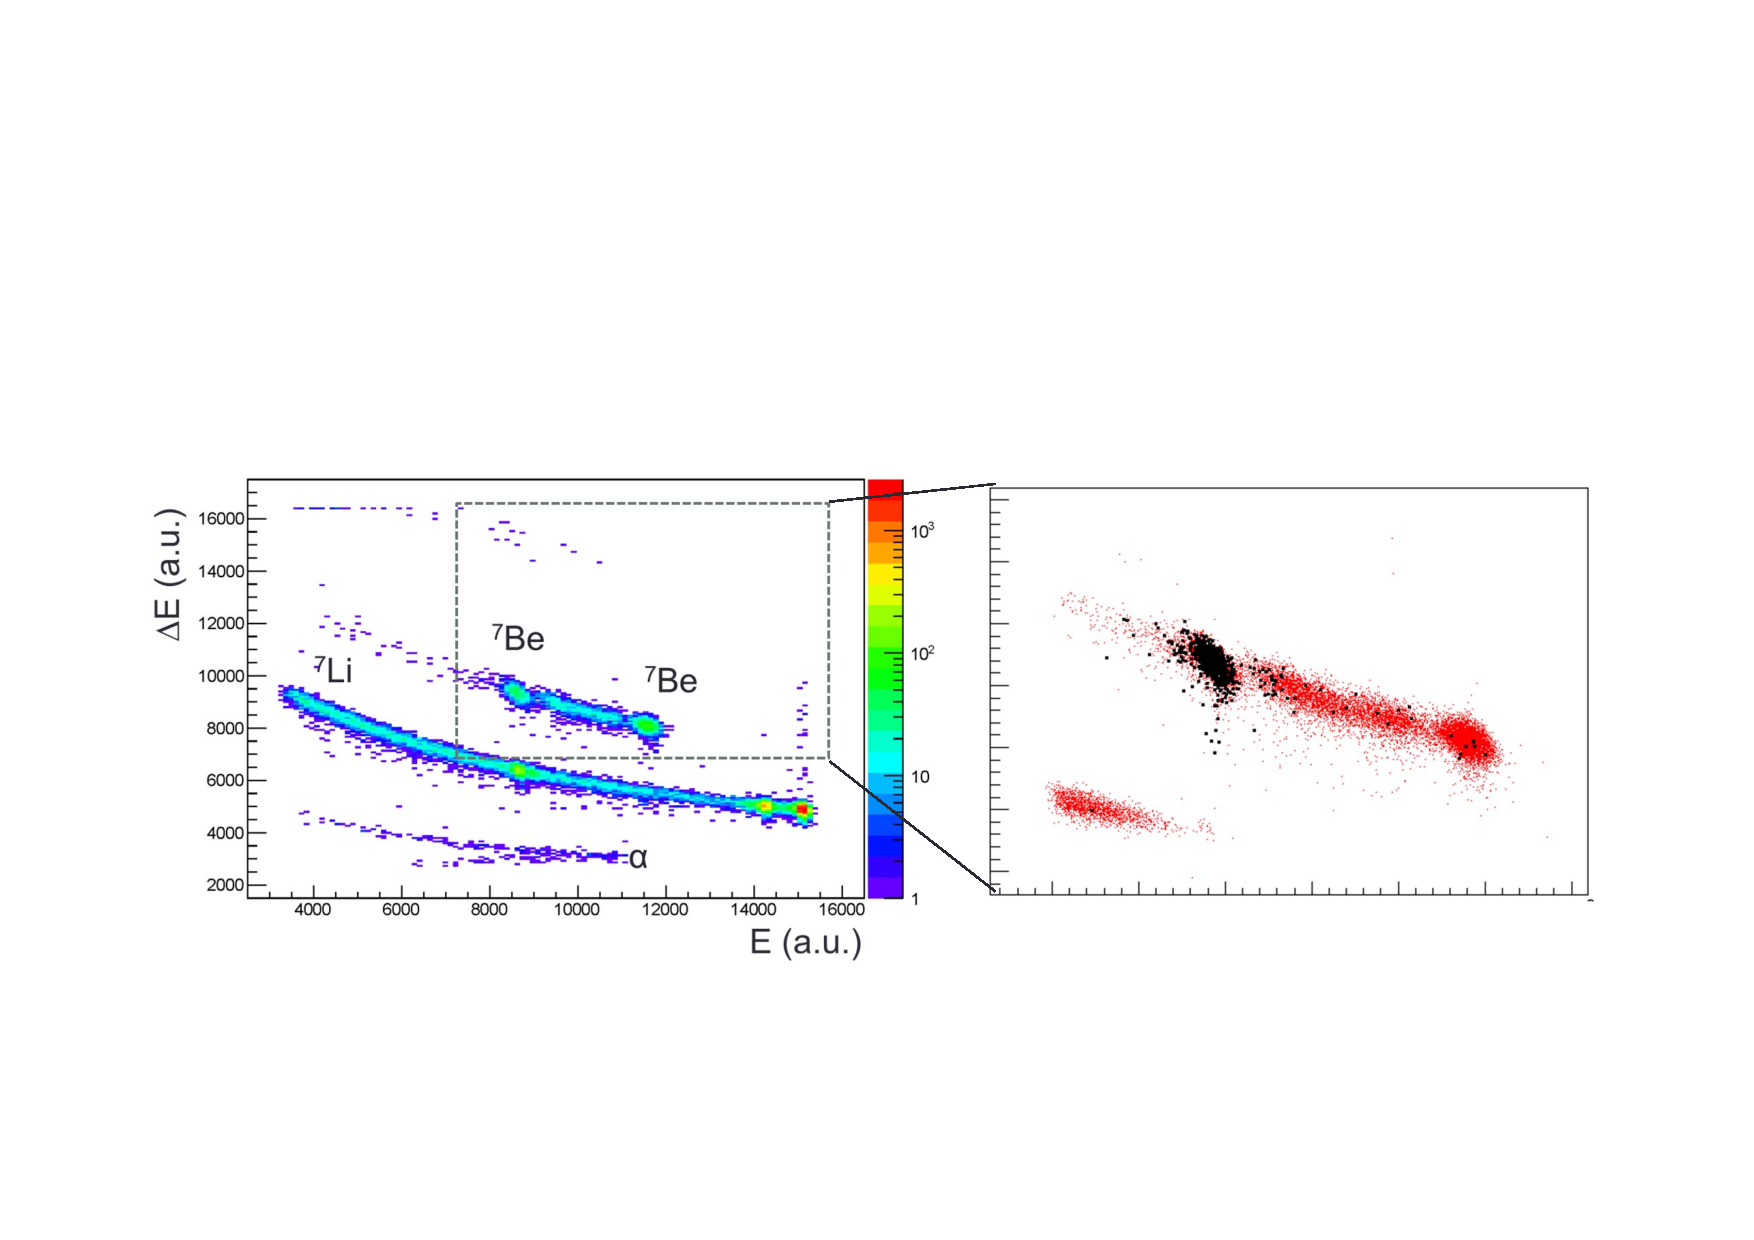
\includegraphics[width=\columnwidth]{./Figures/SiData_Li.pdf}
\caption[Preliminary data from the \ReD\ experiment]{{\bf Left:} scatter plot of the amplitudes of the $\Delta E$ and $E$ Si detectors, placed at 5~deg with respect to the beam axis. {\bf Right:} zoom of the previous scatter plot in the region of the $^{7}$Be \emph{loci}; the black markers are events having a coincident signal in the \TPC.}
\label{fig:bananaplot}
\end{figure}

After another LNS test beam in September 2018, the ReD TPC has been transported back to Naples, to complete the characterization and re-commissioning in the lab there. Tests have been performed to characterize the basic TPC performance in terms of light yield, uniformity, electric field configuration and S2/S1 ratio in double phase. The system was calibrated with ordinary $\gamma$-sources and with an internal $^{83m}$Kr source, which generates a uniform distribution of mono-energetic events.  Activities are still ongoing to characterize the extraction and multiplication fields. A campaign was also carried out at LNS to measure the neutron detection efficiency of the liquid scintillators, using a fission $^{252}$Cf source.  A test beam for the characterization of the neutron beam is going to be performed at LNS in June 2019 and for this run only the Si detectors and the LSci detectors will be deployed.  

The ReD project has received scientific approval by the Scientific Committee of LNS (PAC) for a five-week beam allocation that is granted for 2019.  Upon completion, the \ReD\ \LArTPC\ will be transported back to Catania and a new beam run with the full setup will be scheduled.